%! TEX root = ../main.tex
\documentclass[../main.tex]{subfiles}

\begin{document}

\section{Rumore} \label{sec:rumore}

Otturando il sensore in modo che non fosse raggiunto dalla luce sono state raccolte delle misure per stimare il valore della corrente di buio. Facendo una media e una semi-dispersione sono stati ottenuti i valori di intensità: \num{0.030+-0.006} per il fondoscala \textit{lampadina} e \num{0.017+-0.005} per il fondoscala \textit{candela}.

È stato notato come il rumore subisca una notevole variazione cambiando il fondoscala come è possibile notare dalla \autoref{fig:scale 0.04}. Mentre variando l'apertura del sensore si ottiene una diminuzione del rumore inferiore (\autoref{fig:noise 0.04}).

\begin{figure}[ht!]
    \centering
    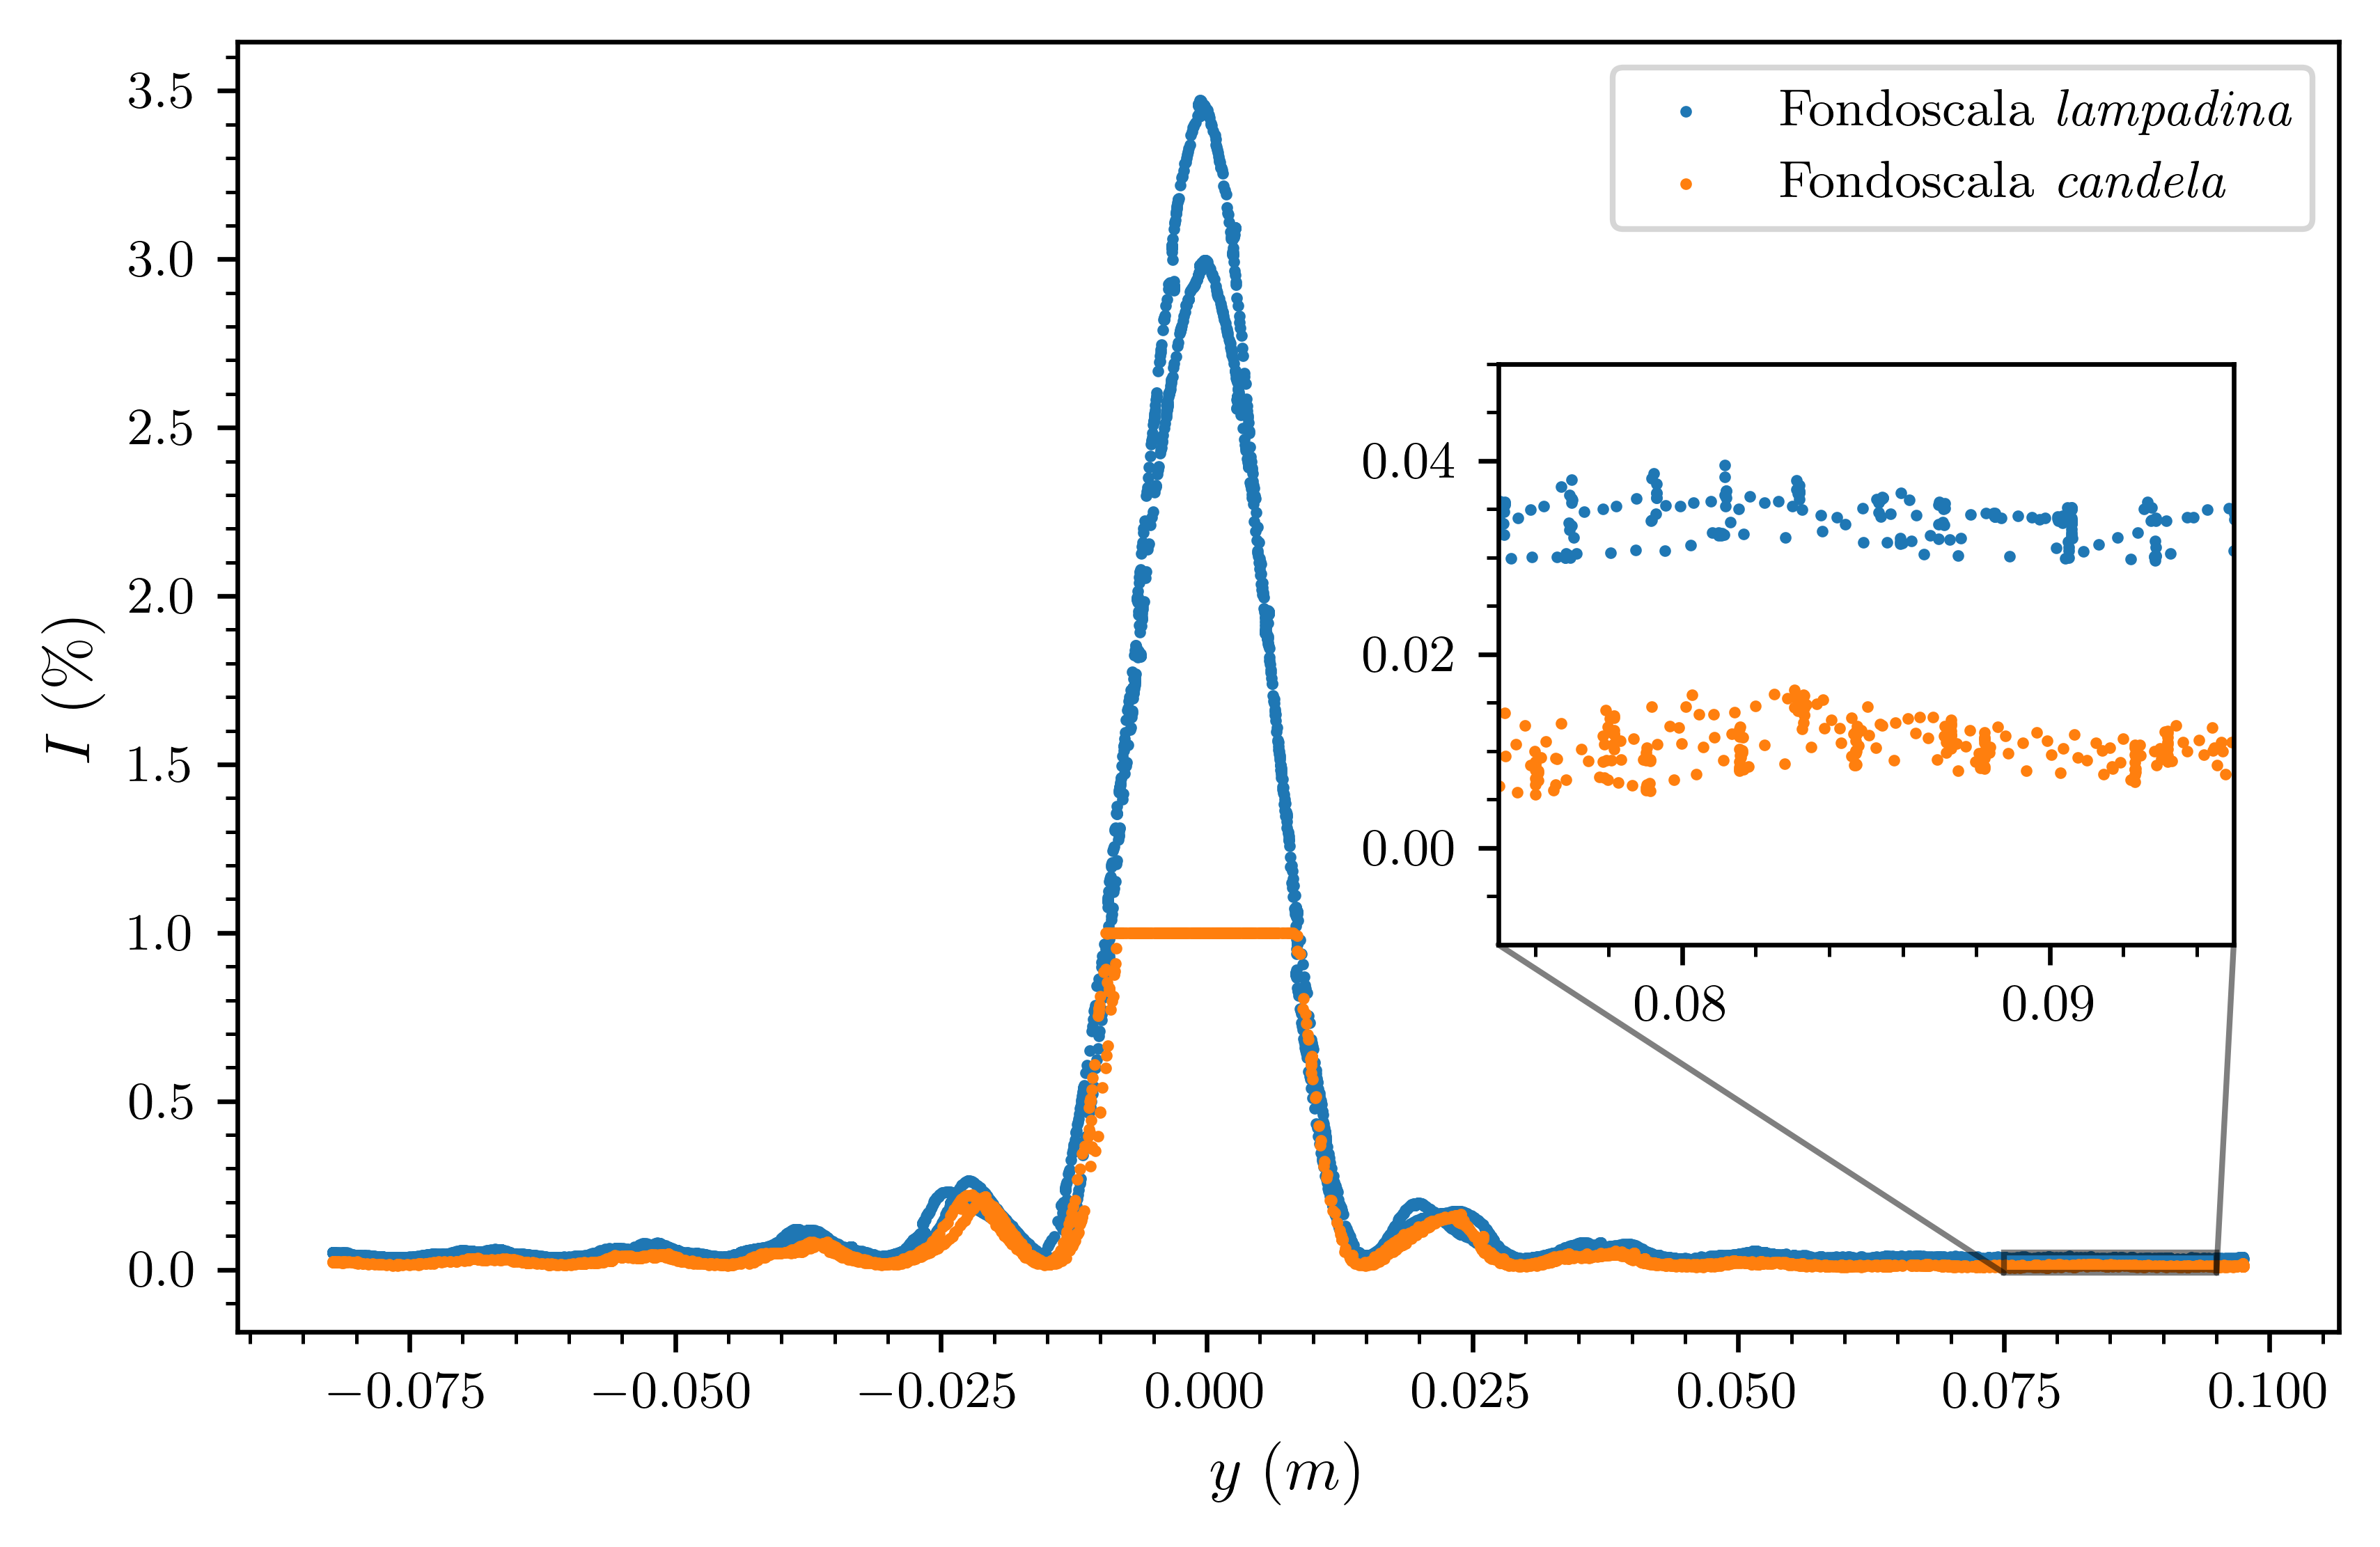
\includegraphics{scale_0.04.png}
    \caption{Grafico dell'intensità luminosa relativa $I$ in funzione della posizione $y$ (in metri) con fenditura a \qty{0.04}{\mm} e apertura del sensore fissata a \qty{1.0}{\mm}. È possibile osservare come il rumore registrato all'estremo della curva sia minore quando si utilizza un fondoscala differente, questo è stato attribuito alla variazione della corrente di buio per i diversi fondoscala che risulta essere \num{0.030+-0.006} per il fondoscala \textit{lampadina} e \num{0.017+-0.005} per il fondoscala \textit{candela}.} %? review: magari aggiungendo come sono state ricavate le misure della corrente di buio e come sono stati stimati gli errori su di esse (come semi-disperione delle misure più grande e più piccola)
    \label{fig:scale 0.04}
\end{figure}

\begin{figure}[ht!]
    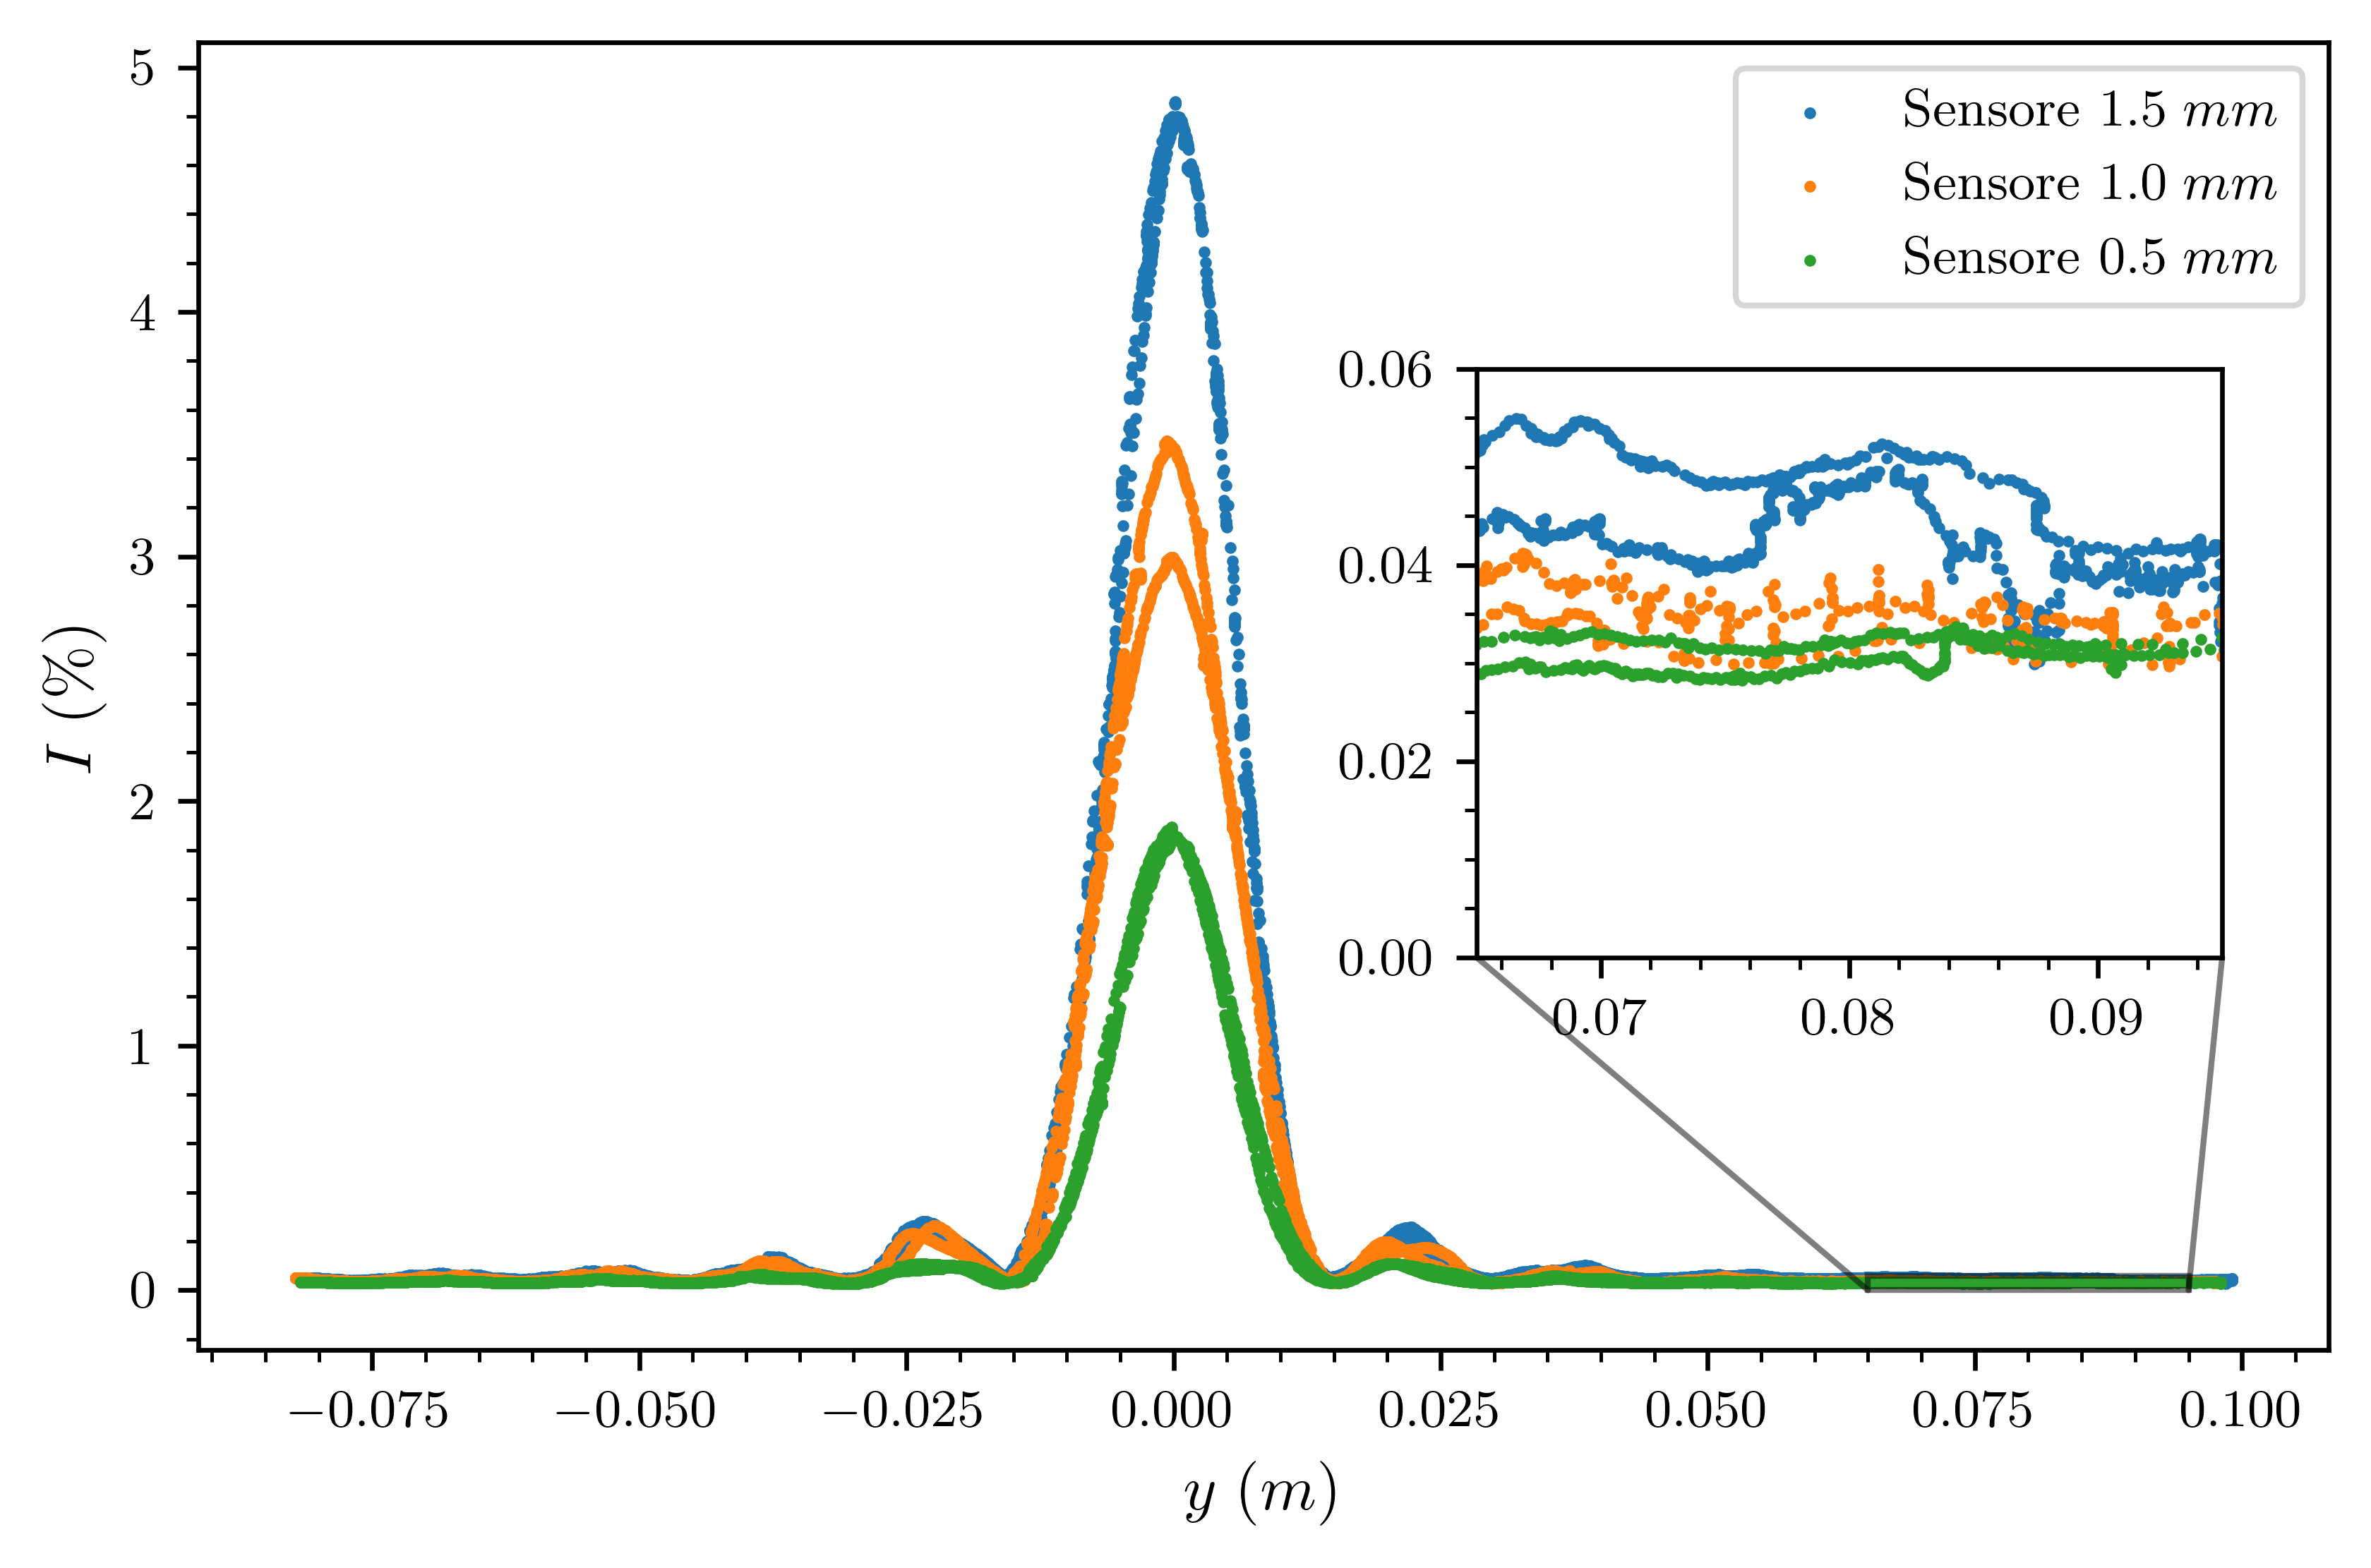
\includegraphics{noise_0.04.png}
    \caption{Grafico dell'intensità luminosa relativa $I$  in funsione della posizione $y$ (in metri) con fenditura \qty{0.04}{\mm} variando l'apertura del sensore. Si nota ccome il rumore diminuisca al diminuire dell'apertura del sensore, tuttavia questa variazione risulta essere inferiore a quella causata dal cambio di fondoscala.}
    \label{fig:noise 0.04}
\end{figure}

\end{document}